%%%%%%%%%%%%%%%%%%%%%%%%%%%%%%%%%%%%%%%%%
% Lachaise Assignment
% LaTeX Template
% Version 1.0 (26/6/2018)
%
% This template originates from:
% http://www.LaTeXTemplates.com
%
% Authors:
% Marion Lachaise & François Févotte
% Vel (vel@LaTeXTemplates.com)
%
% License:
% CC BY-NC-SA 3.0 (http://creativecommons.org/licenses/by-nc-sa/3.0/)
% 
%%%%%%%%%%%%%%%%%%%%%%%%%%%%%%%%%%%%%%%%%


%----------------------------------------------------------------------------------------
%	PACKAGES AND OTHER DOCUMENT CONFIGURATIONS
%----------------------------------------------------------------------------------------

\documentclass{article}

%%%%%%%%%%%%%%%%%%%%%%%%%%%%%%%%%%%%%%%%%
% Lachaise Assignment
% Structure Specification File
% Version 1.0 (26/6/2018)
%
% This template originates from:
% http://www.LaTeXTemplates.com
%
% Authors:
% Marion Lachaise & François Févotte
% Vel (vel@LaTeXTemplates.com)
%
% License:
% CC BY-NC-SA 3.0 (http://creativecommons.org/licenses/by-nc-sa/3.0/)
% 
%%%%%%%%%%%%%%%%%%%%%%%%%%%%%%%%%%%%%%%%%

%----------------------------------------------------------------------------------------
%	PACKAGES AND OTHER DOCUMENT CONFIGURATIONS
%----------------------------------------------------------------------------------------

\usepackage{amsmath,amsfonts,stmaryrd,amssymb} % Math packages

\usepackage{enumerate} % Custom item numbers for enumerations

\usepackage[ruled]{algorithm2e} % Algorithms

\usepackage[framemethod=tikz]{mdframed} % Allows defining custom boxed/framed environments

\usepackage{listings} % File listings, with syntax highlighting
\lstset{
	basicstyle=\ttfamily, % Typeset listings in monospace font
}

%----------------------------------------------------------------------------------------
%	DOCUMENT MARGINS
%----------------------------------------------------------------------------------------

\usepackage{geometry} % Required for adjusting page dimensions and margins

\geometry{
	paper=a4paper, % Paper size, change to letterpaper for US letter size
	top=2.5cm, % Top margin
	bottom=3cm, % Bottom margin
	left=2.5cm, % Left margin
	right=2.5cm, % Right margin
	headheight=14pt, % Header height
	footskip=1.5cm, % Space from the bottom margin to the baseline of the footer
	headsep=1.2cm, % Space from the top margin to the baseline of the header
	%showframe, % Uncomment to show how the type block is set on the page
}

%----------------------------------------------------------------------------------------
%	FONTS
%----------------------------------------------------------------------------------------

\usepackage[utf8]{inputenc} % Required for inputting international characters
\usepackage[T1]{fontenc} % Output font encoding for international characters

\usepackage{XCharter} % Use the XCharter fonts

%----------------------------------------------------------------------------------------
%	COMMAND LINE ENVIRONMENT
%----------------------------------------------------------------------------------------

% Usage:
% \begin{commandline}
%	\begin{verbatim}
%		$ ls
%		
%		Applications	Desktop	...
%	\end{verbatim}
% \end{commandline}

\mdfdefinestyle{commandline}{
	leftmargin=10pt,
	rightmargin=10pt,
	innerleftmargin=15pt,
	middlelinecolor=black!50!white,
	middlelinewidth=2pt,
	frametitlerule=false,
	backgroundcolor=black!5!white,
	frametitle={Command Line},
	frametitlefont={\normalfont\sffamily\color{white}\hspace{-1em}},
	frametitlebackgroundcolor=black!50!white,
	nobreak,
}

% Define a custom environment for command-line snapshots
\newenvironment{commandline}{
	\medskip
	\begin{mdframed}[style=commandline]
}{
	\end{mdframed}
	\medskip
}

%----------------------------------------------------------------------------------------
%	FILE CONTENTS ENVIRONMENT
%----------------------------------------------------------------------------------------

% Usage:
% \begin{file}[optional filename, defaults to "File"]
%	File contents, for example, with a listings environment
% \end{file}

\mdfdefinestyle{file}{
	innertopmargin=1.6\baselineskip,
	innerbottommargin=0.8\baselineskip,
	topline=false, bottomline=false,
	leftline=false, rightline=false,
	leftmargin=2cm,
	rightmargin=2cm,
	singleextra={%
		\draw[fill=black!10!white](P)++(0,-1.2em)rectangle(P-|O);
		\node[anchor=north west]
		at(P-|O){\ttfamily\mdfilename};
		%
		\def\l{3em}
		\draw(O-|P)++(-\l,0)--++(\l,\l)--(P)--(P-|O)--(O)--cycle;
		\draw(O-|P)++(-\l,0)--++(0,\l)--++(\l,0);
	},
	nobreak,
}

% Define a custom environment for file contents
\newenvironment{file}[1][File]{ % Set the default filename to "File"
	\medskip
	\newcommand{\mdfilename}{#1}
	\begin{mdframed}[style=file]
}{
	\end{mdframed}
	\medskip
}

%----------------------------------------------------------------------------------------
%	NUMBERED QUESTIONS ENVIRONMENT
%----------------------------------------------------------------------------------------

% Usage:
% \begin{question}[optional title]
%	Question contents
% \end{question}

\mdfdefinestyle{question}{
	innertopmargin=1.2\baselineskip,
	innerbottommargin=0.8\baselineskip,
	roundcorner=5pt,
	nobreak,
	singleextra={%
		\draw(P-|O)node[xshift=1em,anchor=west,fill=white,draw,rounded corners=5pt]{%
		Question \theQuestion\questionTitle};
	},
}

\newcounter{Question} % Stores the current question number that gets iterated with each new question

% Define a custom environment for numbered questions
\newenvironment{question}[1][\unskip]{
	\bigskip
	\stepcounter{Question}
	\newcommand{\questionTitle}{~#1}
	\begin{mdframed}[style=question]
}{
	\end{mdframed}
	\medskip
}

%----------------------------------------------------------------------------------------
%	WARNING TEXT ENVIRONMENT
%----------------------------------------------------------------------------------------

% Usage:
% \begin{warn}[optional title, defaults to "Warning:"]
%	Contents
% \end{warn}

\mdfdefinestyle{warning}{
	topline=false, bottomline=false,
	leftline=false, rightline=false,
	nobreak,
	singleextra={%
		\draw(P-|O)++(-0.5em,0)node(tmp1){};
		\draw(P-|O)++(0.5em,0)node(tmp2){};
		\fill[black,rotate around={45:(P-|O)}](tmp1)rectangle(tmp2);
		\node at(P-|O){\color{white}\scriptsize\bf !};
		\draw[very thick](P-|O)++(0,-1em)--(O);%--(O-|P);
	}
}

% Define a custom environment for warning text
\newenvironment{warn}[1][Warning:]{ % Set the default warning to "Warning:"
	\medskip
	\begin{mdframed}[style=warning]
		\noindent{\textbf{#1}}
}{
	\end{mdframed}
}

%----------------------------------------------------------------------------------------
%	INFORMATION ENVIRONMENT
%----------------------------------------------------------------------------------------

% Usage:
% \begin{info}[optional title, defaults to "Info:"]
% 	contents
% 	\end{info}

\mdfdefinestyle{info}{%
	topline=false, bottomline=false,
	leftline=false, rightline=false,
	nobreak,
	singleextra={%
		\fill[black](P-|O)circle[radius=0.4em];
		\node at(P-|O){\color{white}\scriptsize\bf i};
		\draw[very thick](P-|O)++(0,-0.8em)--(O);%--(O-|P);
	}
}

% Define a custom environment for information
\newenvironment{info}[1][Info:]{ % Set the default title to "Info:"
	\medskip
	\begin{mdframed}[style=info]
		\noindent{\textbf{#1}}
}{
	\end{mdframed}
}
 % Include the file specifying the document structure and custom commands

\usepackage{pgf}
\usepackage{booktabs}
\usepackage{graphicx}
\usepackage{listings}
\usepackage{hyperref}
\usepackage{wrapfig}
\usepackage{subcaption}

%----------------------------------------------------------------------------------------
%	ASSIGNMENT INFORMATION
%----------------------------------------------------------------------------------------

\title{Assignment 3: Sentiment Analysis with Convolutional Neural Networks} % Title of the assignment

\author{Filip Stefaniuk\\ \texttt{filipste@student.matnat.uio.no}} % Author name and email address

%----------------------------------------------------------------------------------------

\begin{document}

\maketitle
\section*{Introduction}
In this assignment, I have implemented Convolutional Neural Network classifier
based on Kim\footnote{\href{https://arxiv.org/abs/1408.5882}{Yoon Kim 2014}} 2014 and 
Ye Zang\footnote{\href{https://arxiv.org/abs/1510.03820}{Ye Zang et al. 2015}} 2015
work. I haven't achieved the accuracies listed in papers, but I suspect this is due to the
fact that the dataset we have in this assignment is different. The authors of the mentioned
papers used also the \textbf{phrases} part of the SST-2 dataset for training.\\
I have implemented two scripts:
\begin{itemize}
    \item \lstinline{train_model.py} - used for training
    \item \lstinline{eval_on_test.py} - used for evaluation
\end{itemize}
Aditionally I have several functions splitted across the python modules:
\begin{itemize}
    \item \lstinline{data.py} - data preprocessing
    \item \lstinline{emb.py} - loading embeddings and creation of embeddings layers
    \item \lstinline{model.py} - functions for creating the models
\end{itemize}
All the experiments were run on abel with the scripts provided in the \lstinline{scripts}
directory. Source code, scripts, logs from experiments, results as json files,
notebooks used to present the data and sourcecode of this report 
available in github repository\footnote{\href{https://github.uio.no/filipste/INF5820-Assignment3}{https://github.uio.no/filipste/INF5820-Assignment3}}

\section{Baseline sentiment analisys}
I have build CNN model with hyperparameters listed in the assignment, namely:
\begin{enumerate}
    \item categorical cross-entropy loss
    \item pre-trained 300-D \textit{word2vec} embeddings trained on Google News corpus,
    I used original version downloaded from the web.
    \item sequence of static word embeddings
    \item window sizes of 3, 4 and 5
    \item 100-D filters
    \item ReLU activation function
    \item global 1-max pooling
    \item dropout with dropout rate of 0.5
\end{enumerate}
I have not restricted the vocabulary size resulting in having 13295 words in vocabulary.
I have padded and truncated sentences to length of 50. As a result I received architecture listed below.
\newpage
\begin{figure}[h]
    \centering
    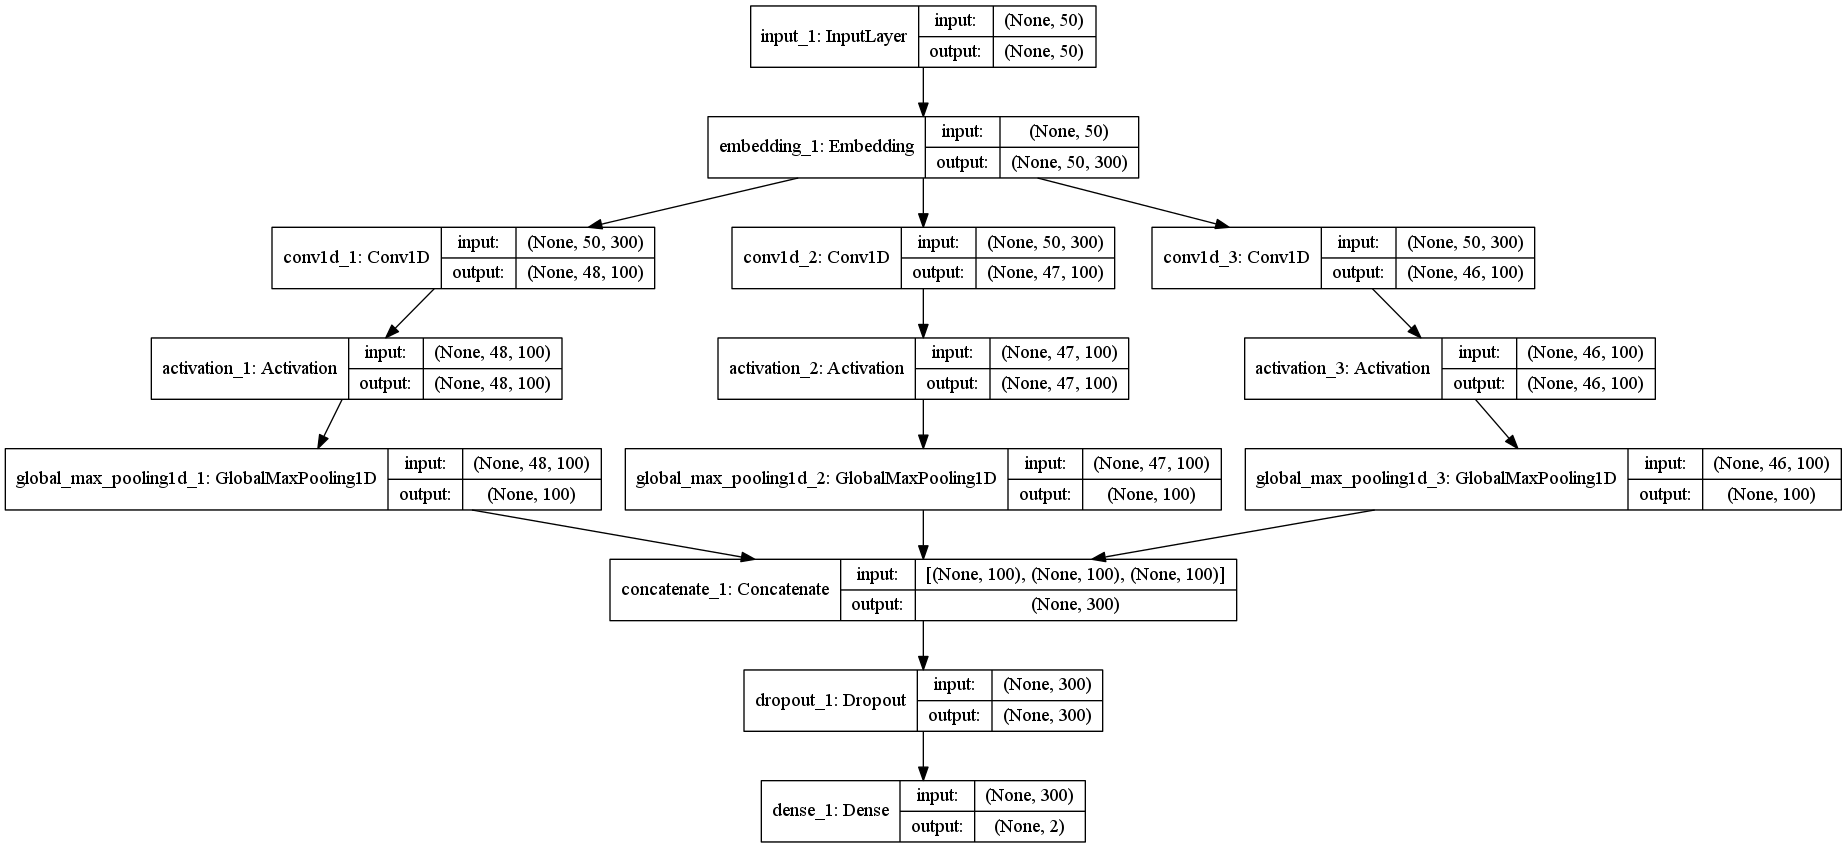
\includegraphics[width=1\textwidth]{../figures/baseline.png}
    \caption{Baseline model architecture}
\end{figure}
I have trained the model using batch size of \textbf{256} and \textbf{adadelta} optimizer 
(same as in the papers).
\section{Controlling the randomness}
I have trained the model 10 times both with unset seed and seed set to \textbf{123}. I got
the following results:
\begin{figure}[h]
    \centering
    \begin{tabular}{lrrrr}
\toprule
{} &    min &    max &   mean &    std \\
\midrule
no seed &  0.767 &  0.783 &  0.777 &  0.006 \\
seed    &  0.776 &  0.799 &  0.789 &  0.007 \\
\bottomrule
\end{tabular}

\end{figure}
Setting the seed doesn't change much, maybe because I am using GPU.
\section{Sensitivity analysis: tuning hyperparameters}
When testing hyperparameters I was changing value of only one of them keeping
the rest as in a baseline model. The authors of the \textit{A Sensitivity Analysis of (and Practitioners’ Guide to) Convolutional
Neural Networks for Sentence Classification} concluded that almost always 1-max pooling strategy
outperformed all the other approches and dropout is the best regularization term. Because of that I decided
that those two hyperparameters are not interesting to test and experimented with all the others.
I set the same seed for all the experiments.


\subsection{Activation function}
\begin{wrapfigure}[9]{r}{0.5\textwidth}
    \begin{center}
        \begin{tabular}{lr}
\toprule
activation &  accuracy \\
\midrule
tanh      &  0.768485 \\
sigmoid   &  0.665455 \\
elu       &  0.780606 \\
relu      &  \textbf{0.793939} \\
leakyrelu &  0.789091 \\
\bottomrule
\end{tabular}

    \end{center}
    \caption{Accuracy with different activations}
\end{wrapfigure}
I have tested multiple activation functions in convolutional layers. The \textit{sigmoid} and 
\textit{tanh} activations performed poorly. I tried different variations of \textit{ReLU} activation
namely \textit{eLU} and \textit{leakyReLU} but there was no improvement. Seems like the \textit{ReLU}
is the best activation function to use in this case, what is similar to the conclusions of authors of 
\textit{A Sensitivity Analysys...} paper.


\newpage
\subsection{Convolutional window size}
I have tested the same window sizes as in the previously mentioned paper,
it seems that in this case there is not much of a difference when using different
window sizes. Turns out that the best setting was either using the 3-4-5, 1-3-5-7 or simply 3 window size.
Seems like window size of 3 is enough to capture necessairy information.

\subsection{Number of filters per window size}
Experimenting with the filter size, yielded results that the optimal size of the filter is 200.
\begin{figure}[h]
    \begin{subfigure}{0.5\textwidth}
        \centering
        \begin{tabular}{lr}
\toprule
window sizes &  accuracy \\
\midrule
1        &  0.787879 \\
1-3-5-7  &  0.792727 \\
14-15-16 &  0.753939 \\
2-3-4    &  0.786667 \\
2-3-4-5  &  0.773333 \\
3        &  \textbf{0.796364} \\
3-4-5    &  0.790303 \\
4-5-6    &  0.780606 \\
5        &  0.773333 \\
6-7-8-9  &  0.761212 \\
7-8-9    &  0.761212 \\
\bottomrule
\end{tabular}

        \caption{Accuracy with different window sizes}
    \end{subfigure}
    \begin{subfigure}{0.5\textwidth}
        \centering
        \begin{tabular}{llr}
\toprule
{} & filter\_size &  accuracy \\
\midrule
0 &          50 &  0.772121 \\
1 &         100 &  0.786667 \\
2 &         200 &  \textbf{0.791515} \\
3 &         300 &  0.790303 \\
4 &         500 &  0.772121 \\
5 &        1000 &  0.785455 \\
\bottomrule
\end{tabular}

        \caption{Accuracy with different filter sizes}
    \end{subfigure}
\end{figure}

\subsection{Raw, lemmatized and POS tagged data}
I have tried using POS tagged data, but it seems that the word embedding model with
POS tags is not good. Using Google News model (\textit{1.zip}) there was \textbf{9001} out of vocabulary tokens,
so the model had very poor results.\\
To compare results when using lemmatized and non-lemmatized data I used models trained on Wikipedia and Gigaword
(\textit{17.zip, 18.zip, 19.zip 20.zip}). There was no clear improvement when using lemmatized data. 


\begin{figure}[h]
    \begin{subfigure}{0.5\textwidth}
        \centering
        \begin{tabular}{lrrr}
\toprule
{} &     f1 &  precision &  recall \\
\midrule
negative &  0.679 &      0.659 &   0.701 \\
positive &  0.666 &      0.688 &   0.645 \\
average  &  0.673 &      0.673 &   0.673 \\
\bottomrule
\end{tabular}

        \caption{Metrics when using model 1.zip}
    \end{subfigure}
    \begin{subfigure}{0.5\textwidth}
        \centering
        \begin{tabular}{lrr}
\toprule
{} &    raw &  lemmatized \\
\midrule
wiki+Gigaword (w2v)   &  0.655 &       0.661 \\
wiki+Gigaword (glove) &  0.753 &       0.765 \\
\bottomrule
\end{tabular}

        \caption{Comparison of using raw and lemmatized data}
    \end{subfigure}
\end{figure}

\subsection{Multiple channels}
I have tested model with multiple channels, one with static and the second with
no-static word embeddings as in Kim 2014. Results are presented in section about
influence of word embeddings.

\newpage
\section{Testing the influence of word embeddings}
I have tested multiple word embeddings in 3 modes: \textbf{static}, \textbf{non-static} and \textbf{multichannel}.
Fine tuning helps achieve better results, but the best scores were achieved when using \textbf{multichannel} mode.
Fasttext turned out to be the best model.
\begin{figure}[h]
    \centering
    \begin{tabular}{lrrr}
\toprule
{} &  static &  non-static &  multichannel \\
\midrule
wiki+Gigaword (w2v)      &   0.655 &       0.659 &         0.704 \\
wiki+Gigaword (glove)    &   0.753 &       0.764 &         0.759 \\
GoogleNews (w2v)         &   0.790 &       0.795 &         0.790 \\
CommonCrawl 840B (glove) &   0.790 &       0.794 &         0.804 \\
wiki-news (fasttext)     &   \textbf{0.796} &       \textbf{0.801} &         \textbf{0.818} \\
\bottomrule
\end{tabular}

    \caption{Comparison of different word embeddings.}
\end{figure}
\subsection{Inferring vectors for OOV words}
Inferring OOV words further improved the results. Model trained with these embeddings achieved
accuracy \textbf{0.818} in \textbf{static} mode.
\begin{figure}[h]
    \centering
    \begin{tabular}{lrrr}
\toprule
{} &     f1 &  precision &  recall \\
\midrule
negative &  0.812 &      0.831 &   0.794 \\
positive &  0.824 &      0.807 &   0.842 \\
average  &  0.818 &      0.819 &   0.818 \\
\bottomrule
\end{tabular}

    \caption{Results after infering OOV words}
\end{figure}

\subsection{Influence of vocabulary size}
I have tested how changing the vocabulary size changes the number of the oov tokens.
Experiments were performed on Google News \textit{w2v}.
\begin{figure}[h]
    \centering
    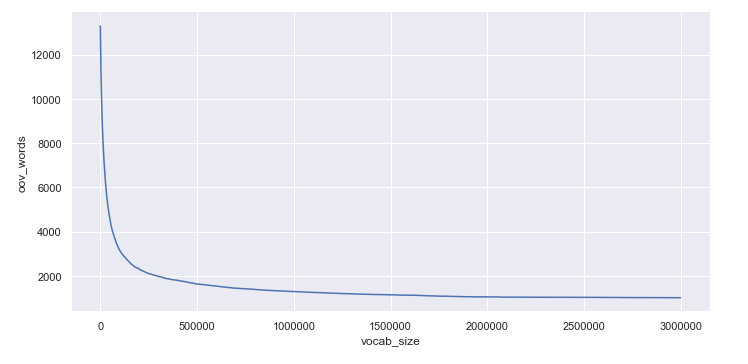
\includegraphics[scale=0.5]{../figures/vocab_size.png}
    \caption{Results after infering OOV words}
\end{figure}

\newpage
\section{Evaluation of the best model}
\end{document}
